\documentclass{article}

\title{Programming Project I, Second Report}
\author{Illya Starikov, Claire Trebing, \& Timothy Ott}
\date{Due Date: March 17, 2016}

\usepackage[final]{pdfpages}

\usepackage{changepage}
\usepackage{wrapfig}
\usepackage{multicol}
\usepackage{booktabs}
\usepackage{amsmath, amssymb}
\usepackage{hyperref}
\usepackage{sidecap}
\usepackage{graphicx}

\hypersetup{
    colorlinks=true,
}

\usepackage{listings}
\usepackage{courier}
\lstset{
  basicstyle=\ttfamily,
  columns=fullflexible,
  keepspaces=true,
}

\newcommand{\ignore}[1]{}
\newcommand{\br}{\multicolumn{2}{c}{} \\}

\begin{document}
\maketitle

\section{Abstract}
As proposed in the first report, we would like to the compare the effeciency of different memory management methods via a \href{https://en.wikipedia.org/wiki/Knapsack_problem#0.2F1_knapsack_problem}{0-1 Knapsack}. We discussed the current memory management methods, the different approaches we would like to use (Brute Force, Dynamic Programming, Greedy Solution) and our plan of implementations.

After implementing the pseudocode provided in Report \#1, rigerous testing and extensive running of sample of data, we have completed conclusive evidence to our proposed problem.

In this report we would like to discuss our findings.

\section{Implementation}
As we discussed in our earlier report we decided to go with a more object-oriented approach to this problem. We created a class called \texttt{App} to represent each application running on our platform. Each instance of the \texttt{App} class contains (as properties\footnote{Or member variables, whatever your preferred notation.}) an identifying number, its memory usage, and its cost to recover from storage. These properties are largely randomized in the construction of each instance. For example, every app has a random memory usage in the range of $32$ to $1028$; the cost is a derived value, taking anywhere from $20$ to $50$ percent of the memory usage of the \texttt{App} in question; we also have a property called \texttt{ratio} which consists of the cost property divided by the memory property and is calculated at creation of the instance by the constructor function, this will be used in our Greedy Algorithm; and lastly each \texttt{App} is given an identifying number based on the index of the cell in the array in which they are initially placed. This ensures that each \texttt{App} will have a unique identifier to help differentiate them whilst\ignore{Sorry, couldn't resist swapping out while for whilst!} checking our solutions against one another.

Initially we considered creating a separate class for our ``\texttt{Smartphone}'' or the platform on which our \texttt{Apps} would be running but later decided against this as this functionality could easily be represented simply by a list (or array) of all the \texttt{Apps}, cutting down on the amount of code we would need.

We implemented our three solutions as one overarching test program that produces arrays of apps in ever increasing input sizes and feeding those arrays to our algorithms one at a time, testing the average runtime over $10$ iterations. The general flow of our program is as follows:

First we specify a list of input sizes that our program will act on, we will discuss this is in more detail further along but for now it should be noted that our first input size is $5$. Our program then creates an array of newly created \texttt{Apps} of the specified input size\footnote{Again, in our first case this is 5.}. These newly created apps have each of their properties randomly assigned by its constructor. Next, because our Greedy Solution requires the inputs be sorted based on its ratio variable and the other solutions do not, we sort the list using Python’s built in sort function.

Now we simply feed the newly sorted list to each of the solution functions in turn, timing the run time of each by taking a timestamp before running the algorithm, again after, then subtracting the two times. We run each program ten times per input and take the average of these for more accuracy. Once each solution algorithm has run ten times the program outputs the data (which includes the solution set, the amount of memory freed by the solution, the combined cost of the solution and the average time it took) to two text files in the directory of the program.

It is at this point that our program returns to the top of the loop for the next input. To ensure a adequate spread of input sizes we defined a list of “base inputs” which we initialized as $5, 10, 15$, and $25$. Once the program finishes iterating over this list, testing each solution as mentioned above, the program returns to the beginning of the input list and multiplies each by 10 to the power of $n$, where $n$ is incremented with each new round of the loop back to the beginning of the base inputs. This entire process is placed in a while loop that is set to infinitely repeat so that we are able to get as many data sets as the program can output in the time we have allotted for testing.

\section{Experiment}
As described above, the tests were run indifferently for a twelve hour period getting our input size to $1,000$. Noting that the for input size of $1,000$ it took the Dynamic Programming approach $1334.81$ seconds, the total time to get accurate results was \textit{3 hours, 42 minutes, and 28 seconds}\footnote{$1334.81$ seconds $\times 10$ iterations $= 13348.1$ seconds = $222.47$ minutes.}. We thought this was a good cut off point.

To ensure accuracy, we decided to run the tests on two machines. These tests can be seen on the graphs, but not the data sets. The tests were fairly comparable, so we decided that displaying data from one data set was sufficient.

We had noticed that the Brute Force was taking a drastically slow time to run (the complexity being $n \times 2^n$). After a sample run, the Brute Force algorithm returned a \texttt{Memory Error} for an input size of $50$. Seeing as we were not likely to be able to have suffecient enough time, we decided to limit the Brute Force to a maximum of $25$ inputs. Below are the results.

\subsection{Results Data Set}
Below you can find the results from our \textit{one of our test}. As stated above, the Brute Force only goes to 25 inputs. Note that the input column is the Input size of applications, the Algorithm is the type of algorithm we used, the Memory was the goal memory we wanted to produce, the Cost was what we wanted to minimize, the Freed is the memory that was actually freed (because we could go over the goal if it was an optimal solution) and finally the Time is the time taken (strictly of the algorithm) measured in seconds.
\begin{adjustwidth}{-.5cm}{}
    \begin{center}
        \begin{tabular}{l|lllll} \toprule
 \textbf{Input} & \textbf{Algorithm} & \textbf{Memory} & \textbf{Cost} & \textbf{Freed} & \textbf{Time} \\ \hline
        & \textsc{Brute}   & 609       & 206.960013686    & 769      &  0.0000652            \\
5       & \textsc{Dynamic} & 609       & 413.920027372    & 1538     &  0.008588             \\
        & \textsc{Greedy}  & 609       & 206.960013686    & 769      &  0.00572586666667     \\ \midrule
        & \textsc{Brute}   & 1254.0    & 306.007083914    & 1307     &  0.0023169            \\
10      & \textsc{Dynamic} & 1254.0    & 913.397426561    & 3126     &  0.033041             \\
        & \textsc{Greedy}  & 1254.0    & 418.629747       & 1961     &  0.0220281            \\ \midrule
        & \textsc{Brute}   & 1896.2    & 462.268333337    & 1980     &  0.0933534            \\
15      & \textsc{Dynamic} & 1896.2    & 706.822856172    & 3129     &  0.10722175           \\
        & \textsc{Greedy}  & 1896.2    & 506.866912451    & 2383     &  0.0714820333333      \\ \midrule
        & \textsc{Brute}   & 2469.0    & 619.523226819    & 2479     &  113.6533167          \\
25      & \textsc{Dynamic} & 2469.0    & 1204.68191427    & 4035     &  56.92951935          \\
        & \textsc{Greedy}  & 2469.0    & 620.454984919    & 2562     &  37.9530137333        \\ \midrule
50      & \textsc{Dynamic} & 5421.2    & 1664.89861527    & 7120     &  0.870269             \\
        & \textsc{Greedy}  & 5421.2    & 1177.03320938    & 5519     &  0.43513695           \\ \midrule
100     & \textsc{Dynamic} & 9783.2    & 2809.24740865    & 11268    &  3.8071061            \\
        & \textsc{Greedy}  & 9783.2    & 2392.11409139    & 9849     &  1.90355725           \\ \midrule
150     & \textsc{Dynamic} & 14995.8   & 4027.50565053    & 16594    &  9.4551353            \\
        & \textsc{Greedy}  & 14995.8   & 3696.37456362    & 15462    &  4.7275798            \\ \midrule
250     & \textsc{Dynamic} & 26793.4   & 6591.81933106    & 28200    &  32.8375575           \\
        & \textsc{Greedy}  & 26793.4   & 6272.26215744    & 27018    &  16.41878765          \\ \midrule
500     & \textsc{Dynamic} & 52354.6   & 12547.9234913    & 53429    &  192.5988691          \\
        & \textsc{Greedy}  & 52354.6   & 12365.0250774    & 52842    &  96.2994775           \\ \midrule
1000    & \textsc{Dynamic} & 107148.2  & 25671.8344823    & 109000   &  1334.8144697         \\
        & \textsc{Greedy}  & 107148.2  & 25256.6939401    & 107895   &  667.4074229          \\
        \bottomrule
        \end{tabular}
    \end{center}
\end{adjustwidth}


\subsection{Results}
While looking at the data we got back, we notice a very noticeable trend immediately: the exponential nature of the quasi-exponential nature of the algorithms. When plotting on an input size vs. graph, we could see even the algorithm with $\mathcal{O}(n)$  (the Greedy Solution) complexity showed some exponential growth. Taking into considering the \href{https://en.wikipedia.org/wiki/Model_of_computation}{RAM Model of Computing} is not completely applicable in this situation, the results are more than staggering.

\begin{adjustwidth}{-1.55cm}{}
    \centering
    \includegraphics[page=2,width=1.25\textwidth]{Graphs.pdf}
\end{adjustwidth}

As can be seen in the above figure, although the input follows the patter of $5n, 10n, 15n, 25n | n \in \mathbb{Z}^+$, the results typically follow a patter of $2\times$ their predecessor.

When comparing the Time vs. Costs, the trend is also quite exponential. For as our algorithms get a larger cost, the time is unquestionably larger. When actually looking at the Time vs. Accuracy, the clear cut winner is Greedy. The time saving are immense compared to Dynamic and Brute Force. On certain cases, Greedy can finish before Dynamic and Brute force combined.

\begin{adjustwidth}{-1.55cm}{}
    \centering
    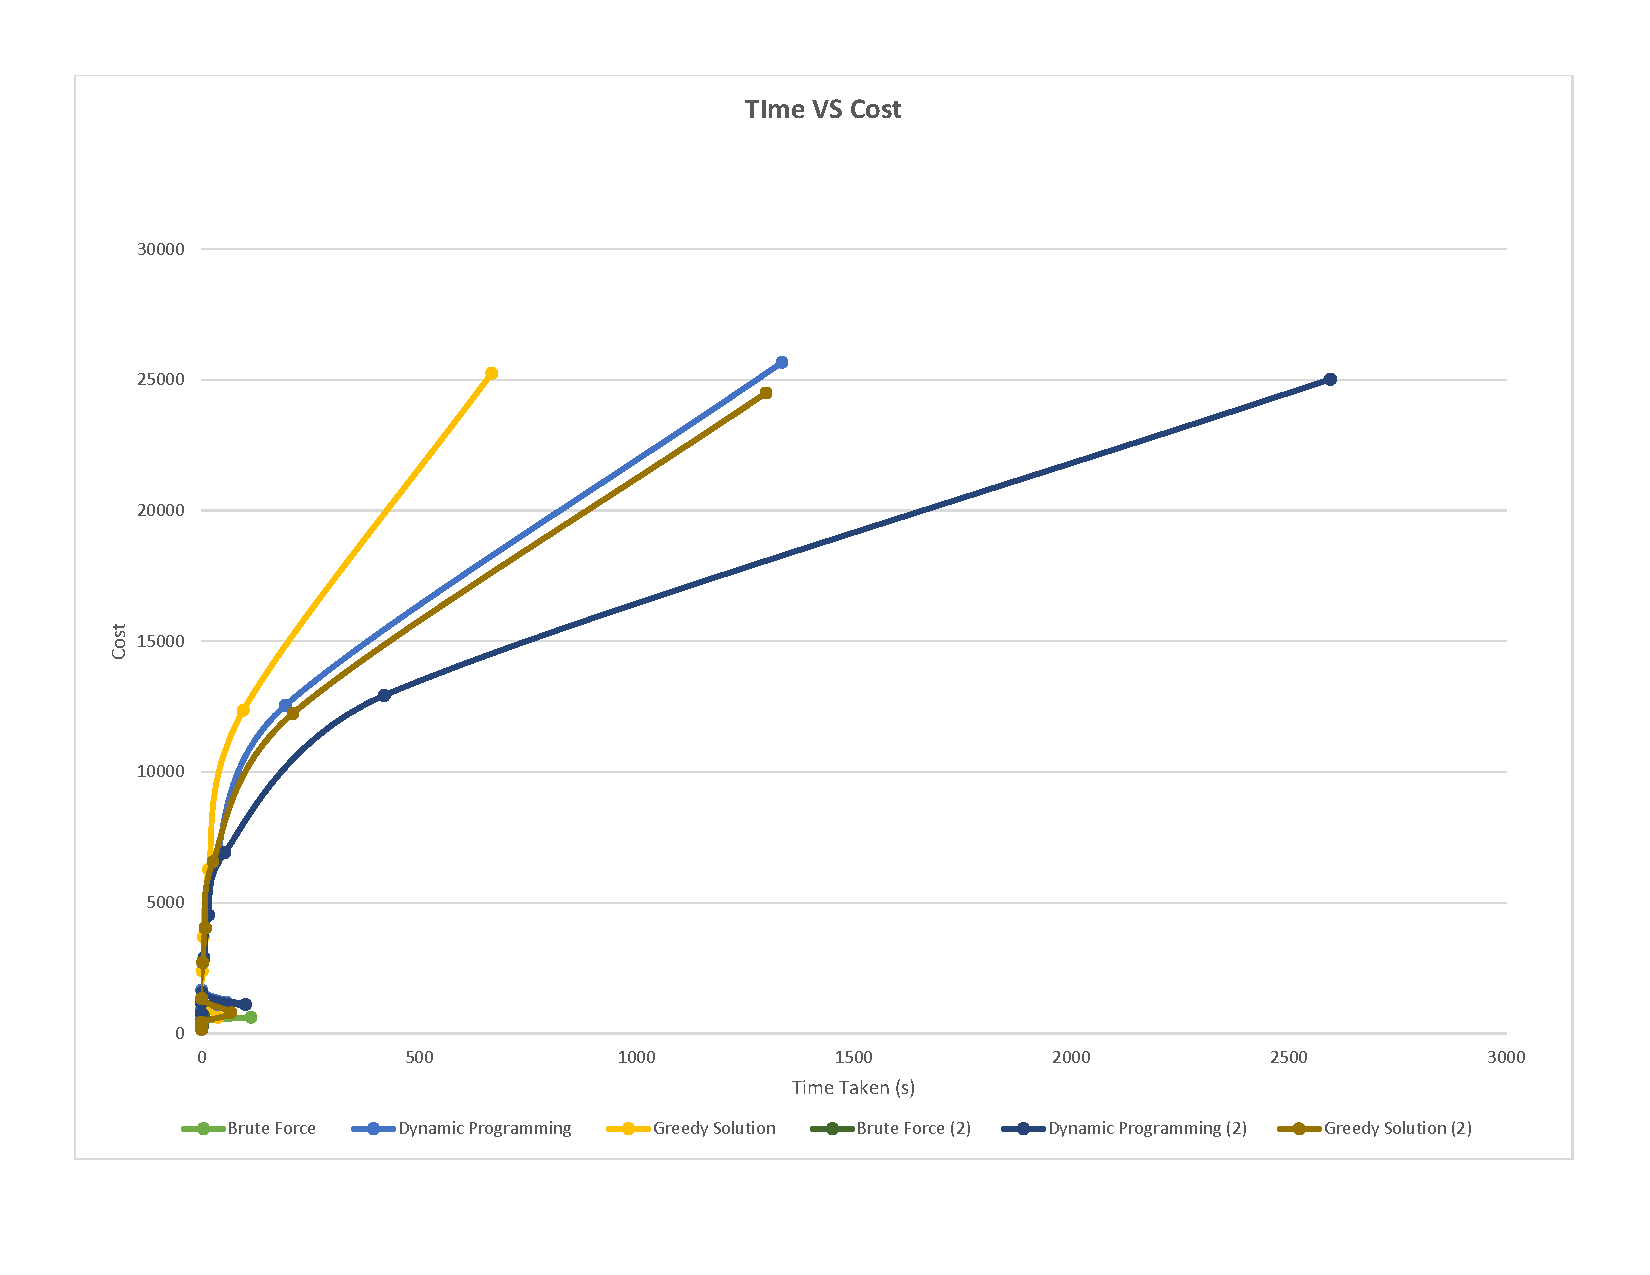
\includegraphics[page=1,width=1.25\textwidth]{Graphs.pdf}
\end{adjustwidth}

We also see that Greedy Solution outperformed the Dynamic in not only time but accuracy. We are unsure of the reasoning behind this, for our algorithm seemed certainly correct on paper.

Tying this back into the real world example, none of these solution would be able to work. Assuming a smartphone of $2GB$ RAM, figuring an optimal solution would take a bare minimum of $38$ seconds (not to mention $2$ minutes if we are using the Brute Force.)

\section{Roles}
\begin{itemize}
    \item Illya Starikov
    \begin{itemize}
        \item Project Manager
        \item Brute Force Development
        \item Abstract, Experiment Writement
    \end{itemize}
    \item Timothy Ott
    \begin{itemize}
        \item Greedy Algorithm Development
        \item Development Writeup
        \item Testing Documents
    \end{itemize}

    \item Claire Trebing
    \begin{itemize}
        \item Dynamic Programming Development
        \item Experiment Writing Up
        \item Quality Assurance
    \end{itemize}
\end{itemize}

\section{Interesting Results}
\section{Conclusion}

\end{document}